%!TEX root = ../thesis.tex
%*******************************************************************************
%****************************** Second Chapter *********************************
%*******************************************************************************

\chapter{The LHC and the CMS Experiment}

\section{The Large Hadron Collider}

The LHC \cite{1748-0221-3-08-S08001} is a circular proton proton accelerator with a circumference of $27 \; \mathrm{km}$ that is designed for a collision energy of $\sqrt{s} = 14 \; \TeV$.
This analysis uses data of proton proton collisions taken in 2016 where the LHC reached a center of mass energy of $\sqrt{s}= 13 \; \TeV$.
The protons are assembled in bunches and accelerated to an energy of  $450 \; \GeV$ by various pre-accelerators before being injected into the LHC.
The two beams in the LHC run in opposite directions and are led by 2136 superconducting dipole magnets.

Colissions are induced at four points along the ring of the LHC. The four main experiments are situated at these interaction points.
The ALICE (A Large Ion Collider Experiment) experiment is designed for heavy ion collisions resulting in events with a very high track multiplicity.
LHCb (Large Hadron Collider beauty) is focused on heavy flavour and forward physics.
The two multi purpose experiments ATLAS (A Toroidal LHC apparatus) and CMS (Compact Muon Solonoid) are designed to deal with a large amount of colisions and
the LHC is designed to deliver more luminosity for these two experiments.

\begin{figure}[htbp!]
  \begin{center}
      \resizebox{0.32 \textwidth}{!}{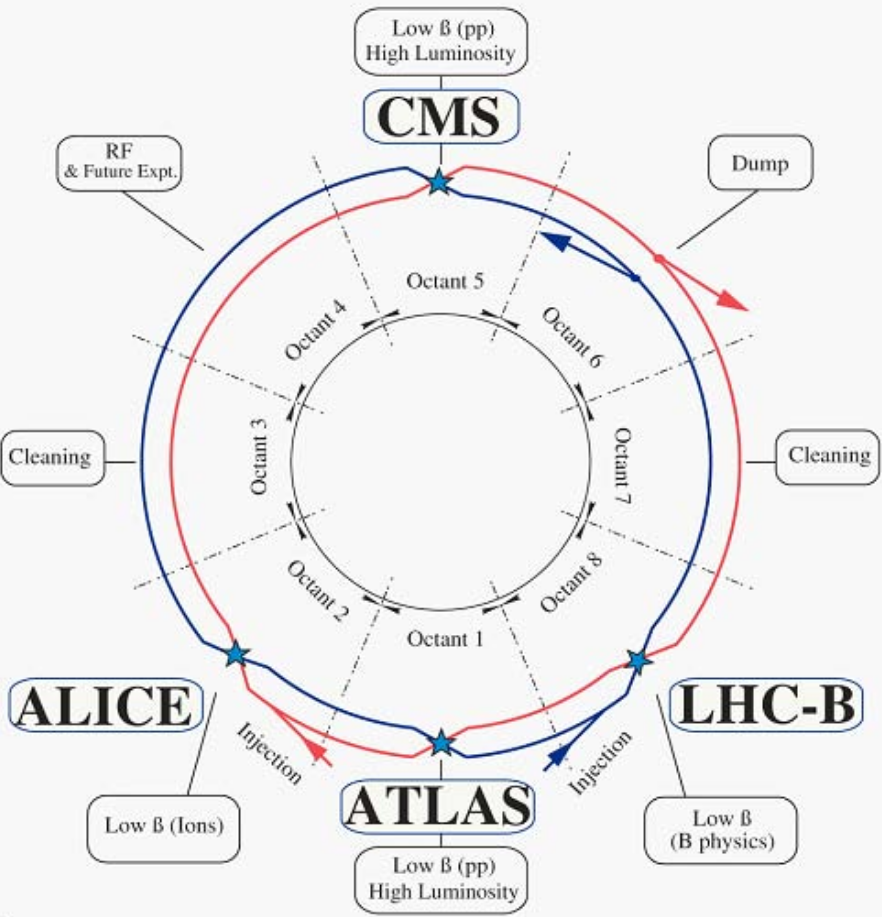
\includegraphics{Detector/Figures/LHC.png}}

\caption{Schematic of the LHC ring showing the two beams as well as the four major experiments. It also shows the injection points as well as the cleaning point and the beam dump. \cite{1748-0221-3-08-S08001}
  \label{fig:det_LHC}}
  \end{center}
\end{figure}

The instantaneous luminosity $\mathcal{L}$ is a measure for the rate of delivered collisions.
It is related to the rate of events $\dot N$ of a process $k$ through the cross section $\sigma_k$:

\begin{equation}
\dot N_k = \mathcal{L} \cdot \sigma_k.
\end{equation}

The luminosity itself can be calculated from the beam properties as given in Equation \ref{}.

\begin{equation}
\mathcal{L} = \frac{N_b \cdot N_p^2 \cdot v}{A}
\end{equation}

Here, $N_b$ stands for the number of bunches, $N_p$ for the number of protons per bunch and $A$ for the profile of the two beams at the interaction.
\todo{different Formula ??}

This analysis uses \lumiv of data taken at a center of mass energy of $\sqrt{s} = 13 \TeV$.

\section{The CMS Detector}

The CMS  detector 

\subsection{The Tracking System}

\subsection{Electric and Hadronic Calorimeters}

\subsection{The Muon System}

\subsection{Triggering}


